% !TEX root = ../CINTA-cn.tex
%%%%%%%%%%%%%%%%%%%%%%%%%%%%%%%%%%%%%%%%%%%%%%%%%%%%%%%%%%%%%%%%%%%%
% Author: Libin Wang
% Chapter 9. Isomorphism, Homomorphisms and Quotient Group
% This document was released as open source on 2026-06-18.
% Copyright 2023, Libin Wang. Creative Commons License
% This work is licensed under a Creative Commons Attribution-NonCommercial-NoDerivatives 4.0 International License.
%
%%%%%%%%%%%%%%%%%%%%%%%%%%%%%%%%%%%%%%%%%%%%%%%%%%%%%%%%%%%%%%%%%%%
\chapter{同构，同态与商群}
\label{chap:iso_hom} % Always give a unique label
% use \chaptermark{}
% to alter or adjust the chapter heading in the running head
\begin{introduction}
  \item 同构
  \item 同态
  \item 商群
  \item 第一同构定理
\end{introduction}

\section{同构} 
\label{sec:iso}
% Motivation.
虽然许多不同的群表现为不同的形式，但本质上也许它们是同一种代数结构。如何刻画所谓本质上相同的群结构，
这引出了\emph{同构}（\emph{isomorphism}）这个概念。
给定两个不同的群，如果能在它们所代表的两类群元素中找到一种
双射（单射且为满射），并且在该映射下群元素的群操作得以保持，则称这两个群同构。 

\begin{definition}{同构}{isom}\index{同构}\index{isomorphism} 
	给定群$(\mathbb{G}, \cdot)$和群$(\mathbb{H}, \circ)$，如果存在一种双射$\phi\colon \mathbb{G} \to \mathbb{H}$，
	使得群操作得以保持，即：
	任取$a, b \in \mathbb{G}$，
	\[\phi(a \cdot b) = \phi(a)\circ \phi(b)\]
	称群$\mathbb{G}$与群$\mathbb{H}$同构，并记为$\mathbb{G}\cong \mathbb{H}$。映射$\phi$被称为一种同构映射。
\end{definition}

\begin{remark}
\emph{同构映射}和之后的\emph{同态映射}是人为造出来的字眼。本来，英文的\emph{isomorphism}（同构）
和\emph{homomorphism}（同态）就是指满足特定条件的映射$\phi$，而
表述两个群同构用的是形容词\emph{isomorphic}（\emph{同构的}），表示两个群同态则用的是
形容词\emph{homomorphic}（\emph{同态的}）。因为中文不大容易区分这里的名词与形容词，
所以在表示名词的同构（或同态）时强调它们是\emph{映射}。
\end{remark}

\begin{example}
$\Z_4\cong \langle i \rangle$，因为可以定义以下双射$\phi\colon \Z_4 \to \langle i \rangle$为$\phi(n) = i^n$。
映射$\phi$是单射且为满射，因为：
\begin{align*}
\phi(0) &= 1\\
 \phi(1) &= i\\
 \phi(2) &= -1\\
 \phi(3) &= -i.
\end{align*}
并且，$\phi$保持了群操作，因为：
\[ \phi(m+n) = i^{m+n} = i^m i^n = \phi(m) \phi(n)\text{。}\]
\end{example}

\begin{example}
	给定群$\mathbb{Z}_8^* = \{1, 3, 5, 7 \}$和群$\mathbb{Z}_{12}^* = \{1, 5, 7, 11 \}$，
	可证明$\mathbb{Z}_8^* \cong \mathbb{Z}_{12}^* $，因为可以定义双射$\phi\colon \Z_8^*  \to \Z_{12}^*$ 如下：
		\begin{align*}
		1 &\mapsto 1 \\
		3 &\mapsto 5 \\
		5 &\mapsto 7\\
		7 &\mapsto 11
		\end{align*}
请读者自行验证群操作得以保持。还可以找到这两个群的另一个同构映射吗？
	\end{example}

\begin{proposition}{}{iso_pr}
%\label{prop:iso_pr}
设$\phi\colon \mathbb{G} \to \mathbb{H}$从群$\mathbb{G}$到群$\mathbb{H}$的一种同构映射，则以下命题为真：
\begin{enumerate}
\item $\phi^{-1}\colon \mathbb{H} \to \mathbb{G}$ 也是同构；

\item $\vert \mathbb{G} \vert = \vert \mathbb{H} \vert $；

\item 如果$\mathbb{G}$ 是阿贝尔群，则$\mathbb{H}$也是阿贝尔群；

\item 如果$\mathbb{G}$ 是循环群，则$\mathbb{H}$也是循环群；

\item 如果$\mathbb{G}$有阶为$n$的子群，则$\mathbb{H}$也有阶为$n$的子群。
\end{enumerate}
\end{proposition}

\begin{proof}
留作课后练习。
\end{proof}

%Propositions about Isomorphisms.
 \begin{proposition}{}{iso_Z}
     %\label{prop:iso_Z}
     所有无限阶的循环群都同构于群$\mathbb{Z}$。
 \end{proposition}
     
 \begin{proof}
 	设群$\mathbb{G}$是一个无限阶的循环群，$g\in \mathbb{G}$是生成元。
 	定义$\phi\colon \mathbb{Z} \to \mathbb{G}$ 为 $n \mapsto g^n$。则
 	\[\phi(m+n) = g^{m+n} = g^m g^n = \phi(m)\phi(n)\text{。}\]
 	然后，证明$\phi$是双射，留作课后练习。 \qed
 \end{proof}

% Theorem about Isomorphisms.}
  \begin{proposition}{}{iso_ord_n}
	%\label{prop:iso_ord_n}
		如果$\mathbb{G}$是阶为$n$的循环群，则$\mathbb{G}$同构于$\mathbb{Z}_n$。
  \end{proposition}
	
	\begin{proof}
		设$\mathbb{G}$是阶为$n$的循环群，$g$是生成元。定义$\phi\colon \mathbb{Z}_n \to \mathbb{G}$为$k \mapsto g^k$，
		其中，$0 \leq k < n$。 
		证明$\phi$是一种同构映射，留作课后练习。 \qed
	\end{proof}

% Theorem about Isomorphisms.
	\begin{corollary}{}{iso_ord_p}
		如果$\mathbb{G}$是阶为$p$的有限群，其中$p$是素数，则$\mathbb{G}$同构于$\mathbb{Z}_p$。
	\end{corollary}
	
	\begin{proof}
		由命题~\ref{pro:iso_ord_n}和推论~\ref{cor:ord_prim}直接可得。 \qed
	\end{proof}

% Proposition about Isomorphisms.
	\begin{proposition}{}{eq_class}
	%\label{prop:eq_class}
	群同构关系决定了一种等价关系，将所有的群划分为不同的等价类。
	\end{proposition}

\begin{proof}
	留作课后练习。
\end{proof}
命题~\ref{pro:eq_class}的证明是简单的，然而其内涵颇深刻，它展示了研究群同构的基本意义。
例如，阶为素数的循环群表现形式有多种，在实际应用中包括$\Z_p^*$的素数阶子群，或者
素数阶椭圆曲线群等。利用推论~\ref{cor:iso_ord_p}的结果，无论素数阶群表现有多大差异，我们都可以通过研究加法群$\mathbb{Z}_p$得到
所有素数阶群的属性。
	
以下是一个有趣的、值得大家知道的结论。
%Cayley's Theorem.
	\begin{theorem}{凯莱定理}{cayley}\index{Cayley theorem}
		每一个群都同构于一个置换群。
	\end{theorem}
%20200617	
\begin{proof}
	给定任意一个$n$阶有限群$\mathbb{G}$，例子~\ref{exm:perm_gr}展示如何构造一个$n$阶置换群$\overline{\mathbb{G}}$。
	定义同态映射$\phi\colon \mathbb{G} \to \overline{\mathbb{G}}$为$g \mapsto \lambda_g$。首先验证这是一种双射，即为单射
	且为满射。$\phi$显然是满射。要证单射，只需要证如果给定两个元素$a,b \in \mathbb{G}$，如果$\phi(a) = \phi(b)$，则$a = b$。
	$\phi(a) = \phi(b)$意味着，对任意群元素$g \in \mathbb{G}$，有$\phi(a) (g)= \phi(b)(g)$，即
		\[ag = \lambda_a(g) = \lambda_b(g) = bg\text{，}\]
	因此，根据消去律，$a=b$。最后，可验证群操作得以保持，因为，
		\[\phi(ab) = \lambda_{ab} = \lambda_a \circ \lambda_b = \phi(a) \circ \phi(b)\text{。}\]
	\qed
\end{proof}
凯莱定理暗示，要研究群需要重点研究对称群和置换群。实际上，在许多现有的计算代数系统中都实现了对称群和置换群，比如 Sage 和 GAP 等。

\section{同态} 
\label{sec:homo}
% Homomorphisms.
放松同构的定义，不要求映射为双射，就有了\emph{同态}（\emph{homomorphism}）\index{同态}\index{homomorphism}的定义。
在本书，同态将被视为一种研究同构的实用的工具。

\begin{definition}{同态}{homo}
	给定两个群$(\mathbb{G}, \cdot)$和$(\mathbb{H}, \circ)$，如果存在映射$\phi\colon \mathbb{G} \to \mathbb{H}$
	使得对任意的$a, b\in \mathbb{G}$，群操作得以保持，即：
	\[\phi(a \cdot b) = \phi(a)\circ \phi(b)\]
	则称群$(\mathbb{G}, \cdot)$同态于群 $(\mathbb{H}, \circ)$。
	映射$\phi$被称为同态映射。
\end{definition}

%Examples of Homomorphisms.
\begin{example}
$\Z$是加法群，定义映射$\phi\colon \Z \to \Z$为$\phi(k) = 2k$，$\forall k \in \Z$。
可以验证$\phi$是一种群同态，它把整数映射为偶数。偶数在加法下成群。
\end{example}

\begin{example}
		设$\mathbb{G}$是群，$g\in \mathbb{G}$。
		定义映射$\phi\colon \Z \to \mathbb{G}$为$\phi(n) = g^n$，$\forall n \in \Z$。
		则$\phi$是一种群同态映射，因为
		\[\phi(m+n) = g^{m+n} = g^m g^n = \phi(m) \phi(n)\text{。}\]
		$\phi$不是一种从$\Z$到$\mathbb{G}$的满射，也不是单射。
		它把$\Z$满射到由$g$生成的$\mathbb{G}$的循环子群。 
\end{example}
	
\begin{example}
		设$p$为素数，任取$g\in \mathbb{Z}_p^*$。请定义映射$\phi\colon \mathbb{Z} \to \mathbb{Z}_p^*$使得$\phi$是
		一种群同态映射。满足何种属性的$g$可使得$\phi$将$\mathbb{Z}$满射到循环群$\mathbb{Z}_p^*$？%可参考例~\ref{exm:cyc_z11}。
\end{example}

\begin{example}
        设$p$为素数，定义映射$\phi\colon \mathbb{Z}_p^* \to \mathbb{Z}_p^*$为$\phi(g) = g^2$，$\forall g\in\mathbb{Z}_p^*$。
        可验证，$\phi$是一种同态映射，因为对任意的$g_1, g_2 \in \mathbb{Z}_p^*$满足：
        $\phi(g_1 g_2) = (g_1 g_2 )^2 =  g_1^2 g_2^2 = \phi(g_1) \phi(g_2)$。
\end{example}

在深入讨论同态之前，先给出一种重要的定义。
\begin{definition}{正规子群}{normal_subg}
		群$\mathbb{H}$是群$\mathbb{G}$ 的子群。如果对任意$g \in \mathbb{G}$，有$g\mathbb{H} = \mathbb{H}g$，
		则称$\mathbb{H}$是群$\mathbb{G}$的正规子群（normal subgroup）\index{normal subgroup}。
\end{definition}
正规子群就是一种使得左陪集与右陪集相等的子群。等式$g\mathbb{H} = \mathbb{H}g$表达某种意义上的“交换律”，
然而对于阿贝尔群，该性质显然成立。请注意，等式$g\mathbb{H} = \mathbb{H}g$并不意味说,
对任意的$g \in \mathbb{G}$，存在$h \in \mathbb{H}$使得$gh = hg $。而是说
对任意的$g \in \mathbb{G}$和$h \in \mathbb{H}$，存在$h' \in \mathbb{H}$使得$g h = h'g$。

%20191027 afternoon.	
\begin{proposition}{}{nor_subg}
设$\mathbb{G}$是群，$\mathbb{H}$是$\mathbb{G}$的子群。以下命题等价。
\begin{enumerate}
\item 子群$\mathbb{H}$是$\mathbb{G}$的正规子群，即对任意$g \in \mathbb{G}$，$g\mathbb{H} = \mathbb{H}g$。

\item 对任意$g \in \mathbb{G}$，有$g\mathbb{H}g^{-1} = \mathbb{H}$。
\end{enumerate}
\end{proposition}

\begin{proof}
$(1)  \implies (2).$ 因为$\mathbb{H}$是$\mathbb{G}$的正规子群，所以对任意$g \in \mathbb{G}$，$g\mathbb{H} = \mathbb{H}g$；
即对任意给定的$g\in \mathbb{G}$和$h \in \mathbb{H}$，存在$h' \in \mathbb{H}$使得$gh=h'g$。
根据消去律，$ghg^{-1} = h' \in \mathbb{H}$，即得$g\mathbb{H}g^{-1} \subseteq \mathbb{H}$。
对任意$h \in \mathbb{H}$，根据以上结论，对任意群元$g^{-1} \in \mathbb{G}$，有$g^{-1}hg = g^{-1}h(g^{-1})^{-1} \in \mathbb{H}$。
因此，存在$h' \in \mathbb{H}$，使得$g^{-1}hg = h'$。所以，$h = gh'g^{-1} \in g\mathbb{H}g^{-1}$，
即$\mathbb{H} \subseteq g\mathbb{H}g^{-1}$。

$(2) \implies (1).$假设对任意$g \in \mathbb{G}$，$g\mathbb{H}g^{-1} = \mathbb{H}$。那么，
对任意$h \in \mathbb{H}$，存在$h'\in \mathbb{H}$使得$ghg^{-1} = h'$。即$gh = h'g$，
这意味着$g\mathbb{H}\subset \mathbb{H}g$。同理，可证$\mathbb{H}g \subseteq g\mathbb{H}$。
\qed
\end{proof}

% Basic Properties of Homomorphisms.
	\begin{proposition}{}{homo}
		设$\phi\colon \mathbb{G}_1 \to \mathbb{G}_2$ 为一种从群$\mathbb{G}_1$到群$\mathbb{G}_2$的群同态映射，则以下命题为真。
		\begin{enumerate}
			\item 如果$e$是$\mathbb{G}_1$的单位元，则$\phi(e)$是$\mathbb{G}_2$的单位元；
			
			\item 对任意群元$g \in \mathbb{G}_1$，$\phi(g^{-1}) = \lbrack \phi(g)\rbrack^{-1}$；
			
			\item 如果$\mathbb{H}_1$是$\mathbb{G}_1$的子群，则$\phi(\mathbb{H}_1)$是$\mathbb{G}_2$的子群；
			
			\item 如果$\mathbb{H}_2$是群$\mathbb{G}_2$的子群，
			则$\phi^{-1}(\mathbb{H}_2) = \{g \in \mathbb{G}_1 : \phi(g) \in \mathbb{H}_2\}$
			是群$\mathbb{G}_1$的子群。
			而且，如果$\mathbb{H}_2$ 是群$\mathbb{G}_2$的正规子群，则$\phi^{-1}(\mathbb{H}_2)$是$\mathbb{G}_1$的正规子群。
		\end{enumerate}
		\qed
	\end{proposition}
	
	\begin{proof}
		\begin{enumerate}
		\item 假设$e$和$e'$分别是群$\mathbb{G}_1$和$\mathbb{G}_2$的单位元，则：
		\[ e'\phi(e) = \phi(e) = \phi(ee) = \phi(e)\phi(e)\]
		然后根据消去律，得到$\phi(e) = e'$。
		
		\item 因为$\phi(g^{-1} )\phi(g)=\phi(g^{-1} g)=\phi(e)=e'$，且$\phi(g) \phi(g^{-1} ) = \phi(g g^{-1}) = \phi(e) = e'$，
		所以，$\phi(g^{-1} ) = \lbrack\phi(g)\rbrack^{-1}$。
		
		\item 首先，$\phi(\mathbb{H}_1)$是非空集合，因为它至少包括群$\mathbb{G}_2$的单位元。任取$a', b' \in \phi(\mathbb{H}_1)$，
		存在$a, b\in \mathbb{H}_1$，使得$\phi(a) = a'$且$\phi(b)=b'$。又因为$\mathbb{H}_1$是$\mathbb{G}_1$的子群，所以有：
		\[ a' b'^{-1} = \phi(a) \lbrack\phi(b)\rbrack^{-1} = \phi(a b^{-1})  \in \phi(\mathbb{H}_1)\]
		最后，根据命题~\ref{pro:subgr}，$\phi(\mathbb{H}_1)$是群$\mathbb{G}_2$的子群。
		
		\item 设$\mathbb{H}_2$是群$\mathbb{G}_2$的子群，记$\mathbb{H}_1 = \phi^{-1}(\mathbb{H}_2)$。首先，$\mathbb{H}_1$
		是非空集合，因为$\phi(e) = e'$，所以，$\mathbb{H}_1$至少包括单位元。任取$a, b \in \mathbb{H}_1$，
		因为$\mathbb{H}_2$是群，则有：
		\[\phi(ab^{-1} )= \phi(a)\lbrack\phi(b)\rbrack^{-1} \in \mathbb{H}_2\]
		因此，$ab^{-1} \in \mathbb{H}_1$，$\mathbb{H}_1$是$\mathbb{G}_1$的子群。
		
		设$\mathbb{H}_2$ 是群$\mathbb{G}_2$的正规子群，要证$\mathbb{H}_1$是$\mathbb{G}_1$的正规子群，即需要证对任意的
		$g\in \mathbb{G}_1$，$h \in \mathbb{H}_1$，有$g^{-1} h g \in \mathbb{H}_1$。因为
		$\mathbb{H}_2$是群$\mathbb{G}_2$的正规子群，所以有：
		\[\phi(g^{-1} h g ) = \phi(g^{-1}) \phi(h) \phi(g) \in \mathbb{H}_2\]
		因此，$g^{-1} h g \in \mathbb{H}_1$。
		\end{enumerate}
		\qed
	\end{proof}

\begin{thinking}
	还记得在第~\ref{chap:group}章中定义的共轭子群吗？
	考虑群$\mathbb{G}$的任意子群$\mathbb{H}$，任取$g \in \mathbb{G}$，构造$g \mathbb{H} g^{-1}$，就得到子群$\mathbb{H}$在$\mathbb{G}$中关于元素$g$的共轭子群。请思考正规子群与共轭子群的关系。
\end{thinking}

		\begin{definition}{kernel}{kernel}
		   	设$\phi\colon \mathbb{G} \to \mathbb{H}$是一种群同态映射，$e$是群$\mathbb{H}$的单位元。根据命题~\ref{pro:homo}，
		   	$\phi^{-1}(\{ e \})$是$\mathbb{G}$的子群，该子群称为$\phi$的 kernel，记为$\Ker\; \phi$。
	\end{definition}
	
	\begin{example}
	        设$p$为素数，同态映射$\phi\colon \mathbb{Z}_p^* \to \mathbb{Z}_p^*$定义为$\phi(g) = g^2$，$\forall g\in\mathbb{Z}_p^*$。
	        可验证，$\phi $把$\{1, p-1\}$映射为
	        群$\phi(\mathbb{Z}_p^*)$的单位元$1$，所以$\Ker\; \phi = \{1, p-1\}$。
	\end{example}
	
		\begin{proposition}{kernel}{kernel}
			设$\phi\colon \mathbb{G} \to \mathbb{H}$是一种群同态映射，则$\phi$的 kernel 是$\mathbb{G}$的正规子群。
	\end{proposition}
	
	\begin{proof}
		 根据命题~\ref{pro:homo}即得，因为$\mathbb{H}$的平凡子群是正规子群。\qed
	\end{proof}

%Quotient group
\section{商群}
\label{sec:quotient_gr}
如果群$\mathbb{H}$是群$\mathbb{G}$的正规子群，则$\mathbb{H}$在$\mathbb{G}$中的陪集形成一个群$\mathbb{G}/ \mathbb{H}$，
群操作是$(a \mathbb{H}) (b \mathbb{H}) = ab \mathbb{H}$。
此群被称为$\mathbb{G}$在$\mathbb{H}$上的\emph{商群}(\emph{quotient group}) \index{quotient group}
或\emph{因子群}(\emph{factor group})\index{factor group}。
通常把$\mathbb{G}/ \mathbb{H}$读成$\mathbb{G}$模$\mathbb{H}$。没错，这里的“模”就是我们之前讲整数同余的那个“$\text{mod}$”，甚至它们具有相同的内涵，可参考第~\ref{chap:cong}章“思考~\ref{thinking:cong}”前后的讨论。该结论可表述为以下定理。

\begin{theorem}{商群}{Quo_Gr}
%\label{thm:Quo_Gr}
若群$\mathbb{H}$是群$\mathbb{G}$的正规子群，则$\mathbb{H}$在群$\mathbb{G}$的陪集形成商群$\mathbb{G}/ \mathbb{H}$，
且群的阶为$\lbrack \mathbb{G}: \mathbb{H}\rbrack$。
\end{theorem}

%Basic ideas of the proof 
现在要证明$\mathbb{G}/ \mathbb{H}$确实是一个群，即要给出定理~\ref{thm:Quo_Gr}的完整证明。证明分为三步：
首先，要理解商群的群操作，即要理解$(a \mathbb{H}) (b \mathbb{H}) = ab \mathbb{H}$的含义。
其次，要证明群操作是一种\emph{良定义}（\emph{well-defined}）操作\index{well-defined}。
最后，验证群公理，这一步最简单。以下分别对这三步骤进行解释。

%Understand the group operation.
理解和证明商群定理的第一步，必须理解商群的群操作，即理解
$(a \mathbb{H}) (b \mathbb{H}) = ab \mathbb{H}$的正确含义。首先，
$(a \mathbb{H}) (b \mathbb{H}) $
是集合的乘法，就是集合中所有元素分别进行群操作所得到的集合。
比如对任意集合$A$和集合$B$进行相乘，得到$AB = \{a b :  a \in A \text{且}  b \in B\}$。
然后，把对该群操作的解释写成以下引理。

\begin{lemma}{}{qgr_op}
群$\mathbb{H}$是群$\mathbb{G}$的正规子群，群$\mathbb{H}$的任意两个陪集$a \mathbb{H}$和$ b \mathbb{H}$
的乘积依然是一个陪集，即
$(a \mathbb{H}) (b \mathbb{H}) = ab \mathbb{H}$。
\end{lemma}
	
\begin{proof}
	因为$\mathbb{H}$是正规子群，所以$a \mathbb{H} = \mathbb{H}a$。
	又因为$\mathbb{H}$是群，所以$\mathbb{H} \mathbb{H}= \mathbb{H}$。因此，
	\[(a \mathbb{H}) (b \mathbb{H}) = (\mathbb{H}a) (b \mathbb{H}) = (a b \mathbb{H}) \mathbb{H} = ab \mathbb{H}\text{。}\]
	\qed
\end{proof}
%20200619
其次，要证明$\mathbb{G}/ \mathbb{H}$中的操作是一种良定义操作，这对于代数的初学者是一个陌生概念。所谓良定义的操作，
就是要求操作独立于所参与操作的\emph{代表元}。比如，对任意群$\mathbb{G}$和其上的某种操作$\psi\colon \mathbb{G}\to \mathbb{G}$，
要求$\psi$良定义就是要求对任意的群元$a, b\in \mathbb{G}$，如果$a = b$，则$\psi(a) = \psi(b)$。第一眼看上去，这个要求很无理，毫无意义，
但是对于商群来说就必不可少。请注意，商群中操作的是陪集，$a\mathbb{H}= b\mathbb{H}$并不意味$a=b$。
而且命题~\ref{pro:coset}强调，每一个陪集中的元素都可以是代表元。那么群操作时使用不同代表元表示的陪集$a\mathbb{H}$
或者$b\mathbb{H}$会不会有不同结果呢？确保群操作的良定义就是要确保群操作独立于陪集的代表元。这种思想表达为以下引理。

\begin{lemma}{商群操作的良定义性}{qgr_op_is_well_defined}
$\mathbb{G}/ \mathbb{H}$中的群操作是一种良定义操作，即如果对任意的群元$a, b, c , d \in \mathbb{G}$，
有$a \mathbb{H} = b \mathbb{H}$且$c \mathbb{H} = d\mathbb{H}$，
则有：
			\[(a\mathbb{H})(c\mathbb{H}) = a c\mathbb{H} = bd \mathbb{H} = (b\mathbb{H})(d\mathbb{H})\]
\end{lemma}

\begin{proof}
根据条件$a \mathbb{H} = b \mathbb{H}$且$c \mathbb{H} = d\mathbb{H}$，则存在 $n_1, n_2 \in\mathbb{H}$，使得
$a = b n_1$，$c = dn_2$。因此，
	\begin{align*}
	ac \mathbb{H} &= b n_1 d n_2 \mathbb{H} \\
	&= b n_1 d \mathbb{H} \\
	&= b n_1 \mathbb{H} d \\
	&= b \mathbb{H} d \\
	&= bd \mathbb{H}
	\end{align*}
又根据引理~\ref{lem:qgr_op}，有$(a \mathbb{H}) (c\mathbb{H}) = ac \mathbb{H}$和
$(b \mathbb{H}) (d\mathbb{H}) = bd \mathbb{H}$，得证。
\qed
\end{proof}
	
最后，完成一些简单工作就可以给出定理~\ref{thm:Quo_Gr}的完整证明。
\begin{proof}
验证$\mathbb{G}/ \mathbb{H}$的群公理，引理~\ref{lem:qgr_op}证明了群操作的封闭性。结合律是显然的。
群的单位元是$e\mathbb{H} = \mathbb{H}$，群元$a\mathbb{H}$的
逆元是$a^{-1}\mathbb{H}$。群的阶就是陪集的个数，即$\lbrack \mathbb{G}: \mathbb{H}\rbrack$。\qed
\end{proof}

以下通过一些简单的例子来熟悉商群。
\begin{example}
		有两种平凡的商群。对任意群$\mathbb{G}$，$e$是它的单位元。商群$\mathbb{G}/\mathbb{G}$同构于平凡群$\{e\}$。
	商群$\mathbb{G}/\{e\}$同构于群$\mathbb{G}$。请读者自行验证。
\end{example}

\begin{example}{（$\mathbb{Z}$的商群）}
群$\mathbb{Z}$是阿贝尔群，所有子群都是正规子群。考虑$\mathbb{Z}$的子群$3\mathbb{Z}$ ，它在$\mathbb{Z}$中的所有陪集是：
		\[0 + 3\mathbb{Z} = \{\ldots, -3, 0, 3, 6, \ldots \}\]
		\[1 + 3\mathbb{Z} = \{\ldots, -2, 1, 4, 7, \ldots \}\]
		\[2 + 3\mathbb{Z} = \{\ldots, -1, 2, 5, 8, \ldots \}\text{。}\]
商群$\mathbb{Z} / 3\mathbb{Z}$的群操作可表述为以下乘法表。
		
\begin{center}
		\begin{tabular}{|c|c|c|c|}
			\hline 
			$+$ & $0 + 3\mathbb{Z}$  & $1 + 3\mathbb{Z}$  &  $2 + 3\mathbb{Z}$\\ 
			\hline 
			$0 + 3\mathbb{Z}$ & $0 + 3\mathbb{Z}$ & $1 + 3\mathbb{Z}$ & $2 + 3\mathbb{Z}$ \\ 
			\hline 
			$1 + 3\mathbb{Z}$& $1 + 3\mathbb{Z}$ & $2 + 3\mathbb{Z}$ & $0 + 3\mathbb{Z}$ \\ 
			\hline 
			$2 + 3\mathbb{Z}$& $2 + 3\mathbb{Z}$ &  $0 + 3\mathbb{Z}$ & $1 + 3\mathbb{Z}$ \\ 
			\hline 
		\end{tabular} 
 \end{center}	
 以上操作可以推广到对任意给定的整数$n$和子群$n\mathbb{Z}$，可得商群$\mathbb{Z}/ n \mathbb{Z}$，请读者自行完成构造。
\end{example}

此时，需要回顾第~\ref{chap:cong}章例~\ref{exam:residue-class}在讲模整数的剩余类时使用的记号，当时提前使用了商群这个概念。之前强调的是“\emph{在同一把尺子（模数）的度量下，将尺寸相同的元素放在同一个集合}，现在在商群的理解中，是强调\emph{使用一个集合(正规子群)来度量某个元素应该放置在什么集合（即陪集，也就是商群的元素）}。借助图~\ref{fig:mod_motivation}可以加深对这种直观的认识，图中$\mathbb{H}$是模数，它度量元素$g$，决定把$g$放到哪一个陪集中。图中的$g$和$g'$落在相同的陪集，也可以理解为$g \equiv g' \pmod{\mathbb{H}}$，也就是$g^{-1} g' \in \mathbb{H}$，参考第~\ref{chap:coset}章的命题~\ref{pro:coset}和课后练习第~\ref{exe:coset}题。这两种理解本质相同，然而后者更具广泛的意义，前者只关心整数，而后者可以扩展到任意的群结构。

%Motivation of First Isomorphism Theorem. 20260521
\begin{figure}[htbp]
	\begin{center}
		\resizebox{0.4\linewidth}{!}{%
		   \input{figures/coset_in_group.tikz}
	    }
		\caption{商群中“模”的直观理解.}
		\label{fig:mod_motivation}       % Give a unique label
	\end{center}
\end{figure}
%20260521

	
\begin{example}{（$\mathbb{Z}_n^*$的商群）}
\label{exm:quo_gr_Zn}
设$n = 15$，则$\mathbb{Z}_n^* = \{ 1, 2, 4, 7, 8, 11, 13, 14\}$。设$g = 2$，记$\mathbb{S} = \langle g \rangle = \{1, 2, 4, 8\}$，
它是$\mathbb{Z}_n^*$的子群。则$\mathbb{Z}_n^* / \mathbb{S} = \{ \mathbb{S}, 7\mathbb{S} \}$，
请验证$\mathbb{S}$是群的单位元，$7\mathbb{S} $的逆元是自己本身，即$(7\mathbb{S}) (7\mathbb{S})  = 4 \mathbb{S}= \mathbb{S}$。
这个例子中有一个特别需要大家注意的要点，同一个群元素可能有不同的表现形式，比如，$7\mathbb{S}$和$14 \mathbb{S}$是同一个陪集。
这也说明了确保群操作良定义的必要性。
\end{example}

\begin{example}{(非良定义操作与商群)}
初学者对良定义操作往往比较疑惑，除了担心良定义本身，通常还会问，难道会有\emph{非良定义}的操作吗？
以下给出一种非良定义操作。设有限循环群$\mathbb{G}=\langle g \rangle$，$\mathbb{H}$是群$\mathbb{G}$的子群，自然也是
正规子群，于是形成商群$\mathbb{G}/\mathbb{H}$。定义映射$\phi_g\colon \mathbb{G}/\mathbb{H} \to \Z $，对任意的$a\mathbb{H}$，
如果$a = g^k$，则$\phi_g(a\mathbb{H}) = k$。可以验证这是一种非良定义映射。

比如，设$p = 7$，则$\mathbb{Z}_p^* = \{ 1, 2, 3, 4, 5, 6\}$，取生成元$g = 3$。记$\mathbb{S} = \{1, 6\}$，
可验证$\mathbb{S}$是$\mathbb{Z}_p^*$的子群。所以形成商群，
$\mathbb{Z}_p^* / \mathbb{S} = \{ \mathbb{S}, 2\mathbb{S}, 3\mathbb{S} \}$。
此时$3\mathbb{S}= 4 \mathbb{S}$，$\phi_3 ( 3 \mathbb{S}) = 1$，但是$\phi_3 (4\mathbb{S}) = 4$。
也就是说，对同一个陪集，因为选取了不同的代表元，得到的映射值不同，该操作不能独立于代表元的选取。
\end{example}

%Isomorphism Theorem
% 20200621
\section{同构定理}
\label{sec:Iso_Thm}
上述知识点可以形成这样一条知识链：从一个群同态$\phi\colon \mathbb{G}_1 \to \mathbb{G}_2$出发。
首先可以找到$\phi$的 kernel，于是得到一个$\mathbb{G}_1$的正规子群；接着，
构造$\mathbb{G}_1$上的商群$\mathbb{G}_1 / \Ker\; \phi$。这一节接着讨论所得商群的性质。
有教材说，这里是通过商群来研究同态。有趣的是，本节所有的例子似乎都是在用同态来研究商群，或者得到商群
相关的性质。而这种性质竟然主要是关于同构，本章第一节的内容。
于是，同构定理把同构、同态、kernel、正规子群和商群等概念紧密地联系起来，成为这条知识链的最重要一环。

%自然同态或者标准同态
%Canonical Homomorphism.
\begin{definition}{标准同态}{can_homo}
	设$\mathbb{H}$是群$\mathbb{G}$的正规子群，定义同态映射$\phi\colon \mathbb{G} \to \mathbb{G} / \mathbb{H}$为$\phi(g) = g \mathbb{H}$，
	$\forall g \in \mathbb{G}$。
    并称该映射为\emph{标准同态}或者\emph{自然同态}（canonical homomorphism），且$\Ker\; \phi = \mathbb{H}$。 
    \index{标准同态}\index{自然同态}\index{canonical homomorphism}
\end{definition}
可以验证，$\phi$确实是一种同态，因为：
\[ \phi(g_1 g_2) = g_1 g_2  \mathbb{H} = g_1  \mathbb{H} g_2  \mathbb{H} = \phi(g_1)\circ \phi(g_2)\]
%First Isomorphism Theorem.
\begin{theorem}{第一同构定理}{first_iso}\index{第一同构定理}\index{first isomorphism theorem}
%\label{thm:first_iso}
如果$\psi\colon \mathbb{G} \to \mathbb{H}$是一种群同态映射，且$\mathbb{K} = \Ker\; \psi$，
则$\mathbb{K}$是$\mathbb{G}$的正规子群。设$\phi\colon  \mathbb{G} \to \mathbb{G} / \mathbb{K}$是标准同态，
则存在唯一同构映射$\eta\colon  \mathbb{G} / \mathbb{K} \to \psi(\mathbb{G})$使得$\psi = \eta \phi$，即$\psi$是
$\eta$和$\phi$的复合映射。
\end{theorem}
%Intuition.
让我们先从表面上理解这个定理。首先，通过群同态映射$\psi\colon \mathbb{G} \to \mathbb{H}$得到一个$\mathbb{G}$的正规子群$\mathbb{K}$，
这是最容易理解的部分。接着，用群$\mathbb{G} $模$\mathbb{K}$得到一个商群$\mathbb{G} / \mathbb{K}$，我们的任务是要
求出该商群的阶。要达到这个目标，定理最后告诉我们，可以找到商群$\mathbb{G} / \mathbb{K}$与$\mathbb{H}$上的子群$\psi(\mathbb{G})$
之间的一个同构映射。注意一点，映射$\psi$并不要求是满射，根据命题~\ref{pro:homo}，$\psi$打到$\mathbb{H}$上的像形成子群$\psi(\mathbb{G})$。
以上思想可以表达为如图~\ref{fig:FIT}的直观图形。

%20230530
%First Isomorphism Theorem.
\begin{figure}
\begin{center}

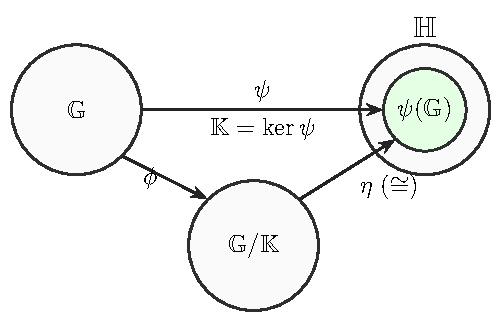
\includegraphics[width=0.6\textwidth]{figures/FIT-fig-improved.pdf}
\caption{第一同构定理的图形化表达}
\label{fig:FIT}      
\end{center}
\end{figure}

为了进一步建立直观，请看图~\ref{fig:FIT_motivation}。已知$\mathbb{K}$中元素都会映射到$\mathbb{H}$的单位元$e$，因为$\mathbb{K}$是 kernel。如果对任意给定元素$g \in \mathbb{G}$，得到一个陪集$g\mathbb{K}$，请问$g\mathbb{K}$的元素会被投影到哪里？提示，$g\mathbb{K}$中的元素是什么形式，当作用到$\psi$之后，根据$\psi$的性质，会得到什么样的变换？

%Motivation of First Isomorphism Theorem. 20260511
\begin{figure}
	\begin{center}
		\input{figures/g_to_h_mapping.tikz}
		\caption{关于第一同构定理的直观认识.}
		\label{fig:FIT_motivation}       % Give a unique label
	\end{center}
\end{figure}
%20260511

%Proof ideas.
有了以上的直观，可以开始定理的证明，证明分为三步。首先，
定理既然是要找一个从$\mathbb{G}/\mathbb{K}$到$\psi(\mathbb{G})$ 同态映射，那就使用构造法，先构造一个同态映射$\eta$。
第二步，证明映射$\eta$是良定义映射。
第三步，证明映射$\eta$是同态且是双射，即为同构映射。以下展示具体证明的细节。

\begin{proof}
		\begin{enumerate}
		\item 定义映射$\eta\colon \mathbb{G}/\mathbb{K} \to \psi(\mathbb{G})$为$\eta(g \mathbb{K}) = \psi(g)$。
		
		\item 证明$\eta$是良定义映射，即证明如果对于两个不同的$g_1, g_2 \in \mathbb{G}$，有$g_1 \mathbb{K}  =  g_2\mathbb{K} $，
		则$\eta(g_1 \mathbb{K} ) = \eta(g_2 \mathbb{K} )$。
		因为$g_1 \mathbb{K}  =  g_2\mathbb{K}$，则存在$k\in \mathbb{K}$使得$g_1 = g_2 k$，这仅仅利用了陪集相等的定义。因此：
		\[ \eta(g_1\mathbb{K} ) = \psi(g_1) = \psi(g_2 k) = \psi(g_2)\psi(k) = \psi(g_2) =  \eta(g_2\mathbb{K})\]
		请注意，上式中第四个等号之所以成立是因为$k\in \mathbb{K}$，而$\mathbb{K}$是$\psi$的 kernel，$k$必然映射到$\mathbb{H}$的单位元。
		这就证明了$\eta$映射独立于陪集代表元的选择。之所以$\eta$是唯一定义的，因为给定了$\psi$和$\phi$，而$\psi = \eta \phi$，且$\phi$是一种满射。%加入是满射的要求是在思考后，并用DeepSeek验证后的结果。2025年4月14日晚。
		
		\item 可证明$\eta$是同态且是双射。$\eta$是同态，因为：
		\begin{align*}
			\eta(g_1\mathbb{K} g_2 \mathbb{K}) &= \eta(g_1 g_2 \mathbb{K}) \\
			&=  \psi(g_1 g_2) \\
			&= \psi(g_1)\psi(g_2)\\
			&= \eta(g_1\mathbb{K})\eta(g_2\mathbb{K})
			\end{align*}
		$\eta$显然是满射，最后，只需证明$\eta$是单射。任取$g_1\mathbb{K}, g_2\mathbb{K}$，
		假设$\eta(g_1\mathbb{K} ) = \eta(g_2\mathbb{K} )$，
		则$\psi(g_1) = \psi(g_2)$。$g_1$和$g_2$是$\mathbb{G}$中两个不同的元素，所以
		\[\psi(g_1) = \psi(g_2 g_2^{-1} g_1) = \psi(g_2) \psi(g_2^{-1} g_1)\]
		即$\psi(g_2^{-1} g_1)$是$\psi(\mathbb{G})$的单位元，也即$g_2^{-1} g_1 \in \mathbb{K}$。
		所以$g_2^{-1} g_1\mathbb{K} = \mathbb{K} $，最后得到$g_1\mathbb{K} = g_2\mathbb{K}$。
		\end{enumerate} \qed
\end{proof}
最后，小结第一同构定理的本质。给定从群$\mathbb{G}$到群$\mathbb{H}$的同态映射$\psi$，
记$\mathbb{K} = \Ker\; \psi$。
目标是求$\psi(\mathbb{G})$中元素的个数，为此构造出商群$\mathbb{G}/\mathbb{K}$与$\psi(\mathbb{G})$的同态映射$\eta$，
从而通过求商群$\mathbb{G}/\mathbb{K}$的阶来得到答案。
以上证明过程显示，任取$g_1\mathbb{K}, g_2\mathbb{K} \in \mathbb{G}/\mathbb{K}$，
如果$\eta(g_1\mathbb{K} ) = \eta(g_2\mathbb{K} )$，则$\psi(g_1) = \psi(g_2)$。这说明落在同一个陪集$g\mathbb{K}$中的
元素都映射到$\psi(\mathbb{G})$中的同一个点$\psi(g)$。所以，$\psi(\mathbb{G})$中元素的个数就是商群$\mathbb{G}/\mathbb{K}$
中元素的个数，也即$|\mathbb{G}|/|\mathbb{K}|$。

\begin{example}{(循环群)}
\label{exm:cyc_gr}
设$\mathbb{G}$是由生成元$g$生成的循环群。定义映射$\phi\colon \Z \to \mathbb{G}$为$n \mapsto \ g^n$， $\forall n \in \Z$。
$\phi$是同态映射，因为：
\[\phi(m + n) = g^{m+n} = g^m g^n = \phi(m) \phi(n)\text{。}\]
$\phi$显然是满射。如果$\mathbb{G}$的阶为$m$，因为$g$是生成元，则$\operatorname{ord}(g) = m$。
于是，$g^m = e$，且有$\Ker\; \phi = m \Z$。根据第一同构定理，则有：
\[\Z / \Ker\; \phi = \Z / m \Z \cong \mathbb{G}\text{。}\]
如果$\mathbb{G}$是无限阶，则$g$也是无限阶，则$\Ker\; \phi = \{ 0 \}$，则$\Z$与$\mathbb{G}$同构。
因此，两个循环群同构当且仅当它们有相同的阶。在同构的意义上，只有两种循环群：$\Z$和$\Z_n$。
\end{example}

\begin{example}{(从$\Z_p^*$到$\Z_p^*$的同态.)} 
	\label{exm:homo_zp}
	设$p$是素数，$\Z_p^*$是循环群。定义映射$\phi\colon \Z_p^* \to \Z_p^*$为$\phi(g) = g^2$，$\forall g \in \Z_p^*$。
	$\phi$是一种群同态映射，因为：
	\[\phi(g_1  g_2) = (g_1 g_2)^ 2 = g_1^2 g_2^2 = \phi(g_1) \phi(g_2)\]
	显然，$\phi$不是满射，且$\Ker\; \phi = \{1, p-1\}$是$\Z_p^*$的一个正规子群。知道$\Ker\; \phi$是因为
	根据命题~\ref{pro:inv_mod_prime}，以下公式
	\[x^2 \equiv 1 \pmod{p}\]
    有且仅有两个解，即 $1$和 $p-1$。
	验证可知$\mathbb{S} = \{ \phi(g): g \in\Z_p^*\} $是群。群$\mathbb{S}$的阶是多少？
	根据第一同构定理，$\vert \mathbb{S} \vert = \vert \Z_p^* /  \Ker\; \phi \vert =  \vert \Z_p^* \vert /  2$。
\end{example}

\begin{example}{(从$\Z_n^*$ 到$\Z_n^*$的同态.)} 
	\label{exm:homo_zn}
	设$n = p q$是合数，$p$和$q$是素数，则$\Z_n^*$是群。定义映射$\phi\colon \Z_n^* \to \Z_n^*$为$\phi(g) = g^2$，
	$\forall g \in \Z_n^*$。可验证$\phi$是一种群同态映射。记$\mathbb{S} = \{ \phi(g):  g \in\Z_n^*\}$。
	如果知道$\Ker\; \phi$的阶，则根据第一同构定理，可知$\vert\mathbb{S} \vert =\vert \Z_n^* \vert /  \vert \Ker\; \phi \vert $，
	要完成这个目标，需要知道以下公式有多少个解：
	\[ x^2 \equiv 1 \pmod{n}\]
	可惜，命题~\ref{pro:inv_mod_prime}并不能完成这个任务，需留待第~\ref{chap:crt}章再解决这个问题。
\end{example}
	
\begin{example}
\label{exm:signed_gr}
设$n$是一个正整数。对所有的$x \in \Z_n$，定义$\vert x \vert$为求$x$的绝对值，其中$x$表达为$\{ -(n-1)/2, \ldots, (n-1)/2\}$范围内的带符号整数。
从群$\Z_n^*$出发，定义集合$\mathbb{G}^+$为
\[\mathbb{G}^+  = \{ \vert x \vert : x \in \Z_n^*\} \]
对$g, h \in \mathbb{G}^+$，定义以下操作
\[ g \circ h = \vert g \cdot h \bmod n \vert\]
可验证$(\mathbb{G}^+, \circ)$ 是一个群。这是第~\ref{chap:group}章的课后习题。
现在，利用第一同构定理，可以解决求该群的阶是多少的问题。

观察可知，取绝对值的操作（不妨记为$\phi$）是一种从$\Z_n^*$到$\mathbb{G}^+$的同态映射，因为：
\[ \phi(x\cdot y) = \vert x \cdot y \vert = \vert x \vert \circ \vert y \vert = \phi(x) \circ \phi(y) \]
又因为$-1 \in \Z_n^*$，所以$\Ker\; \phi = \{1, -1\}$。最后，根据第一同构定理，$\mathbb{G}^+$的阶是
$\vert \Z_n^* \vert / 2 $。
\end{example}

%%%20220714。From ST16第6章
\begin{proposition}{}{r_mod_z_eq_o}
商群$\mathbb{R}/ \mathbb{Z}$同构于圆圈群$\mathbb{O}$（第~\ref{chap:group}章例~\ref{exm:cycle_gr}）。
\end{proposition}

\begin{proof}
定义映射$\phi\colon \mathbb{R} \to \mathbb{O}$为：
\[\phi(x) = e^{2\pi i x}\]
可验证$\phi$是一种满同态，且 kernel 为$\Z$。作为提示，请注意两点。首先，
\[e^{2\pi i x} = \cos(2\pi x) + i \sin(2\pi x)\]
其次，因为$\Z$是加法群，所以，此时$\mathbb{R}$也看为加法群，否则$\Z$就不是$\mathbb{R}$的子群，商群也就无从说起。
\qed
\end{proof}

\begin{thinking}
\label{thk:r_mod_z}
请问，为什么以上证明需要$\phi$是满同态？如何证明$\phi$是一种满同态？
\end{thinking}

%Editted by lbwang on 20191115
%2020062 改写
\begin{definition}{}{dir_prod}
%\label{def:dir_prod}
给定两个群$\mathbb{G}$和$\mathbb{H}$，记$\mathbb{G}\times \mathbb{H}$为集合$\mathbb{G}$与集合$\mathbb{H}$的笛卡尔乘积，并
定义集合$\mathbb{G}\times \mathbb{H}$中元素的乘法操作$\cdot$为：
\[(g_1, h_1) \cdot (g_2, h_2) = (g_1g_2, h_1h_2)\text{。}\]
可验证，$\mathbb{G}\times \mathbb{H}$是群，并称为$\mathbb{G}$与$\mathbb{H}$的
\emph{直积}（\emph{direct product}）\index{直积}\index{direct product} 。
\end{definition}

\begin{definition}{}{dir_sum}
%\label{def:dir_sum}
给定一个阿贝尔群$\mathbb{G}$和它两个子群$\mathbb{H}_1$和$\mathbb{H}_2$，且满足$\mathbb{H}_1 \cap \mathbb{H}_2 = \{ e \}$。
定义$\mathbb{H}_1 \oplus \mathbb{H}_2$为：
\[\mathbb{H}_1 \oplus \mathbb{H}_2 = \{h_1 h_2: h_1 \in \mathbb{H}_1, h_2 \in \mathbb{H}_2\}\text{。}\]
可立即验证$\mathbb{H}_1 \oplus \mathbb{H}_2$是一个群，并称之为$\mathbb{H}_1$与$\mathbb{H}_2$的
\emph{直和}（\emph{direct sum}）
\index{直和}\index{direct sum}。
\end{definition}

\begin{proposition}{}{eq_prod_sum}
给定一个阿贝尔群$\mathbb{G}$，设$\mathbb{H}_1$和$\mathbb{H}_2$是群$\mathbb{G}$的任意两个子群，且
$\mathbb{H}_1 \cap \mathbb{H}_2 = \{ e \}$。定义以下映射：
\[ \phi\colon  \mathbb{H}_1 \times \mathbb{H}_2 \to \mathbb{H}_1 \oplus \mathbb{H}_2 \]
为
\[ (h_1, h_2) \mapsto h_1 h_2\text{。}\]
则映射$\phi$是一种同构映射。
\end{proposition}

\begin{proof}
需证明映射$\phi$是同态映射，且是双射。映射$\phi$是同态映射，因为：
\[ \phi((g_1, g_2)\cdot(h_1, h_2)) = \phi(g_1 h_1, g_2h_2) =  g_1h_1g_2h_2 = \phi(g_1,g_2)\phi(h_1, h_2)\text{。}\]
读者可自行体会，为什么需要$\mathbb{G}$是阿贝尔群。
由定义，映射$\phi$显然是满射，只需证它是单射。为此，需证$\Ker\; \phi = \{ (e, e) \}$。
对任意$(g_1, g_2) \in \mathbb{H}_1 \times \mathbb{H}_2$，有$\phi(g_1, g_2) = e $当且仅当
$g_1  g_2 = e$，即$g_1 = g_2^{-1}$。又因为$\mathbb{H}_1 \cap \mathbb{H}_2 = \{ e \}$，因此只能是$g_1 = g_2 = e$。
\qed
\end{proof}

\begin{thinking}
为什么要通过第一同构定理来证明映射$\phi$的单射性，而不直接利用单射的属性？
\end{thinking}
命题~\ref{pro:eq_prod_sum}的证明展示了第一同构定理的威力，然而其结论也有着较深刻的内涵：阿贝尔群的直积与直和同构。因此，
可将阿贝尔群的直积与直和视为同一种代数结构。直白而言，群$\mathbb{G} = \mathbb{H}_1 \oplus \mathbb{H}_2$的
任意元素$g$都具有$ h_1h_2$的形式，即$g$可唯一分解为来自$\mathbb{H}_1$和$\mathbb{H}_2$的两个分量$h_1$和$h_2$。因此，
把$g$看为$h_1h_2$的形式或者$(h_1, h_2)$的序对形式本质上有什么不同吗？
%% 20220215添加，参考：https://mathworld.wolfram.com/GroupDirectSum.html
%%和https://math.stackexchange.com/questions/2450766/the-confusing-nature-of-direct-sum-for-finite-abelian-groups/2451432

%Second Isomorphism Theorem.
利用第一同构定理，轻易地得到了以下第二同构定理，证明很容易，难的只是要阅读。
该定理的目标很直接，给定群$\mathbb{G}$，探讨$\mathbb{G}$的子群$\mathbb{H}$（不必然是正规子群）与正规子群$\mathbb{K}$
之间的关系。图~\ref{fig:SIT}列出了第二同构定理所涉及的群结构，以方便大家阅读。

%Second Iso Theorem
% 20230523，源自DF04第98页。 https://tikzcd.yichuanshen.de/#N4Igdg9gJgpgziAXAbVABwnAlgFyxMJZARgBpiBdUkANwEMAbAVxiRAB12BbOnACwBGA4AAkAvpx78hwANJiQY0uky58hFGQAMVWoxZtJvQcIDiCpSux4CRLaQBMu+s1aIO3YzPGLlIDNbqRA6OzvpuHlImchZ+AWq2mqQAzGGuhp7SwuKcAMZ0aEZZMb5WCRokpAAsaQburGK6MFAA5vBEoABmAE4QXEhkIDgQSPYgfDB0UGyQYA1+PX2j1MNIIeOT0+6z8129-Yhjq4jJ1BNTMwS7IIsH68dVZ5uXc6U3+0inQyOIjxsX2yub1uSD+xwArE8AeAgY0xEA
\begin{figure}
\begin{center}
\begin{tikzcd}
                               & \mathbb{G} \arrow[d, no head]                                &                                \\
                               & \mathbb{H}\mathbb{K} \arrow[ld, no head] \arrow[rd, no head] &                                \\
\mathbb{H} \arrow[rd, no head] &                                                              & \mathbb{K} \arrow[ld, no head] \\
                               & \mathbb{H}\cap\mathbb{K} \arrow[d, no head]                  &                                \\
                               & e                                                            &                               
\end{tikzcd}
\caption{第二同构定理涉及的群结构}
\label{fig:SIT}   
\end{center}
\end{figure}

\begin{theorem}{第二同构定理}{sec_iso}\index{第二同构定理}\index{second isomorphism theorem}
%\label{thm:sec_iso}
$\mathbb{H}$是群$\mathbb{G}$的子群（不必然是正规子群），$\mathbb{K}$是群$\mathbb{G}$的正规子群。
则$\mathbb{H} \mathbb{K}$是群$\mathbb{G}$的子群，$\mathbb{H}\cap \mathbb{K}$是$\mathbb{H}$的正规子群，
且
\[\mathbb{H} / (\mathbb{H}\cap \mathbb{K}) \cong \mathbb{H}\mathbb{K}/\mathbb{K}\text{。}\]
\end{theorem}
%Intuition.
\begin{proof}
该证明包括三部分。第一步，证明$\mathbb{H} \mathbb{K} = \{hk: h \in \mathbb{H}, k \in \mathbb{K}\}$是群$\mathbb{G}$的子群。
$\mathbb{H} \mathbb{K} $显然是非空集合，
任取$h_1 k_1 , h_2 k_2 \in \mathbb{H} \mathbb{K}$，需证$(h_1 k_1)  (h_2 k_2)^{-1} \in \mathbb{H} \mathbb{K}$。
$(h_1 k_1)  (h_2 k_2)^{-1} = h_1 k_1 k_2^{-1} h_2^{-1}$，记$k_1 k_2^{-1} = k'$，
则有：
\[ (h_1 k_1)  (h_2 k_2)^{-1} = h_1 (h_2^{-1} h_2) k' h_2^{-1} = (h_1 h_2^{-1}) (h_2 k' h_2^{-1}). \]
又因为$\mathbb{K}$是正规子群，有
$ h_2 k' h_2^{-1} \in \mathbb{K}$，
所以$(h_1 k_1)  (h_2 k_2)^{-1} \in \mathbb{H} \mathbb{K}$。

第二步，证明$\mathbb{H}\cap \mathbb{K}$是$\mathbb{H}$的正规子群。
根据命题~\ref{pro:nor_subg}的推论（参考课后习题$4$），
只需要证明对任意的$h\in \mathbb{H}$和$k \in \mathbb{H}\cap \mathbb{K}$，$h^{-1} k h \in \mathbb{H}\cap \mathbb{K}$。
但是，结论是显然的，因为$h, k \in \mathbb{H}$，所以$h^{-1} k h \in \mathbb{H}$。又因为$\mathbb{K}$是正规子群，
所以$h^{-1} k h \in \mathbb{K}$。

第三步，定义同态映射$\phi\colon \mathbb{H} \to \mathbb{H}\mathbb{K}/\mathbb{K}$，
对任意的$h\in \mathbb{H}$，$h \mapsto h \mathbb{K}$。然后，验证映射$\phi$是满射，
因为对任意的陪集$hk\mathbb{K}= h\mathbb{K}$，则$h \in \mathbb{H}$是它的原像。再验证$\phi$是同态映射，因为
\[ \phi(hh') =  hh' \mathbb{K} = h\mathbb{K}h'\mathbb{K} = \phi(h)\phi(h').\]

最后，根据第一同构定理，
\[ \mathbb{H}\mathbb{K}/\mathbb{K} = \phi(\mathbb{H}) \cong \mathbb{H}/\Ker\; \phi.\]
又因为
\[\Ker\; \phi = \{ h \in \mathbb{H}: h \in \mathbb{K}\} = \mathbb{H}\cap \mathbb{K} ,\]
所以，$\mathbb{H}\mathbb{K}/\mathbb{K}  \cong \mathbb{H}/(\mathbb{H}\cap \mathbb{K})$。

\qed
\end{proof}

在给出第三同构定理之前，我们先介绍对应定理（\emph{correspondence theorem}），在某些参考书~\cite{DF04}中也称之为“第四同构定理”。对应定理揭示了群 $\mathbb{G}$中包含正规子群$\mathbb{K}$的子群与商群$\mathbb{G}/\mathbb{K}$的子群之间的深层结构对应关系。对应定理蕴含了第三同构定理，尽管证明第三同构定理并不一定需要对应定理。

设$\mathbb{K}$是群$\mathbb{G}$中的正规子群。记$S$为群$\mathbb{G}$中所有包含$\mathbb{K}$的子群的集合，即
$S = \{\mathbb{H}: \mathbb{H} \le \mathbb{G}, \mathbb{K} \le \mathbb{H} \}$。
记$T$为商群$\mathbb{G}/\mathbb{K}$的所有子群的集合，即
$T = \{\mathbb{H}/\mathbb{K}: \mathbb{H}/\mathbb{K} \le \mathbb{G}/\mathbb{K} \}$。我们可以证明集合$S$与集合$T$中的元素存在一一对应关系。即对任意$S$中的元素，$T$中有唯一的元素与之对应，反之亦然。以下等式直观地表示了对应定理：
\[
\{ \text{群}\mathbb{G}\text{中包含正规子群}\mathbb{K}\text{的子群}\} \leftrightarrow \{\text{商群}\mathbb{G}/\mathbb{K}\text{的子群}\}.
\]

\begin{theorem}{对应定理}{corresp_thm}\index{对应定理}\index{correspondence theorem}
 设$\mathbb{K}$是群$\mathbb{G}$中的正规子群。
 定义从集合$S$到集合$T$的映射$\phi$为$\mathbb{H} \mapsto \mathbb{H}/\mathbb{K}$，
 其中$\mathbb{H} \in S$，$\mathbb{H}/\mathbb{K} \in T$。
 那么，$\phi$是一种双射，也就说，集合$S$与集合$T$中的元素一一对应，即
 群$\mathbb{G}$中包含$\mathbb{K}$的子群与商群$\mathbb{G}/\mathbb{K}$的子群一一对应。
 并且，集合$S$中的正规子群与集合$T$中的正规子群一一对应，
 即群$\mathbb{G}$中包含$\mathbb{K}$的正规子群与商群$\mathbb{G}/\mathbb{K}$中的正规子群一一对应。 
\end{theorem}
	
\begin{proof}
首先明确，因为$\mathbb{K}$是群$\mathbb{G}$中的正规子群，那么对任意
包含$\mathbb{K}$的子群$\mathbb{H}$，
$\mathbb{H}/\mathbb{K}$是$\mathbb{G}/\mathbb{K}$的子群。
然后，要证明$\phi$是一种双射，需要分别证明它是单射和满射。

先证明$\phi$是单射。
设$\mathbb{H}_1$和$\mathbb{H}_2$是包含$\mathbb{K}$的$\mathbb{G}$的
子群，且$\mathbb{H}_1/\mathbb{K} = \mathbb{H}_2/\mathbb{K} $，
往证$\mathbb{H}_1 = \mathbb{H}_2$。对任意$h_1 \in \mathbb{H}_1$，
$h_1 \mathbb{K} \in \mathbb{H}_1/\mathbb{K}$，则存在$h_2 \in \mathbb{H}_2$，使得
$h_1 \mathbb{K} = h_2 \mathbb{K}$。即存在$k_1, k_2 \in \mathbb{K}$使得$h_1 k_1 = h_2 k_2$，或$h_1 = h_2 k_2 k_1^{-1}$。
因为$\mathbb{K} \subseteq \mathbb{H}_2$，所以$h_1 \in \mathbb{H}_2$，即$\mathbb{H}_1 \subseteq \mathbb{H}_2$。同理，
$\mathbb{H}_2 \subseteq \mathbb{H}_1$，所以$\mathbb{H}_1 = \mathbb{H}_2$。

其次，证明$\phi$是满射。设$\mathbb{W}$是$\mathbb{G}/\mathbb{K}$的子群。
令$\mathbb{H} = \{g\in \mathbb{G}: g\mathbb{K} \in \mathbb{W}\}$，可证明$\mathbb{H}$是$\mathbb{G}$的子群。
又显然有$\mathbb{K} \subseteq \mathbb{H}$。因此，$\mathbb{W} = \mathbb{H} / \mathbb{K}$，即$\phi$是满射。

要证集合$S$中的正规子群与集合$T$中的正规子群一一对应需要两个方向。
先假定$\mathbb{H}$是$\mathbb{G}$的正规子群，
$\mathbb{K}$是$\mathbb{H}$的子群。
定义映射$\psi\colon \mathbb{G}/\mathbb{K} \to \mathbb{G}/\mathbb{H}$
为$g\mathbb{K} \mapsto g \mathbb{H}$。容易验证，$\psi$是一种同态，
且$\Ker\; \psi  = \mathbb{H}/\mathbb{K} $，
因为%20230529
\begin{align*}
\Ker\; \psi  &=  \{ g\mathbb{K}  \in \mathbb{G}/\mathbb{K} : \psi(g\mathbb{K}) = \mathbb{H}\} \\
                                      &= \{ g\mathbb{K}  \in \mathbb{G}/\mathbb{K} : g\mathbb{H} = \mathbb{H}\} \\
                                      &=  \{ g\mathbb{K}  \in \mathbb{G}/\mathbb{K} : g \in \mathbb{H}\} = \mathbb{H}/\mathbb{K}
\end{align*}
所以$\mathbb{H}/\mathbb{K}$
是$\mathbb{G}/\mathbb{K}$的正规子群。

反方向，设$\mathbb{H}/\mathbb{K}$是$\mathbb{G}/\mathbb{K}$的正规子群，定义以下同态：
\begin{equation}\label{eq:homo}
\mathbb{G} \to \mathbb{G} /\mathbb{K} \to \frac{\mathbb{G} /\mathbb{K}}{\mathbb{H} /\mathbb{K}}
\end{equation}
%\[\mathbb{G} \mapsto \mathbb{G} /\mathbb{K} \mapsto \frac{\mathbb{G} /\mathbb{K}}{\mathbb{H} /\mathbb{K}}\]
此同态的 kernel 是$\mathbb{H}$，因此，$\mathbb{H}$是$\mathbb{G}$的正规子群。要理解以上结论，关键是观察到公式~\ref{eq:homo}
所定义同态的第二个箭头，这也是一种标准同态，它把任意的$g \mathbb{K} $映射为$g (\mathbb{H} /\mathbb{K})$。显然，
所有的$g \in\mathbb{H}$都被映射为$\mathbb{H} /\mathbb{K}$，而这是商群$\frac{\mathbb{G} /\mathbb{K}}{\mathbb{H} /\mathbb{K}}$
的单位元。
\qed
\end{proof}

对应定理的证明已经包含了以下定理的证明。考虑公式~\ref{eq:homo}定义的同态，此同态的 kernel 是$\mathbb{H}$，利用第一同构定理即得。
\begin{theorem}{第三同构定理}{third_iso}\index{第三同构定理}\index{third isomorphism theorem}
%\label{thm:third_iso}
$\mathbb{H}$和$\mathbb{K}$是群$\mathbb{G}$的正规子群，且$\mathbb{K}\le \mathbb{H}$。则：
\[\mathbb{G}/ \mathbb{H} \cong \frac{\mathbb{G}/\mathbb{K}}{\mathbb{H}/\mathbb{K}}\text{。}\]
\end{theorem}
%Intuition.
第三同构定理看上去颇复杂，一种简单的记忆法就是，把符号“$/$”理解为普通除法，$\mathbb{G}/ \mathbb{K}$“除以”$\mathbb{H}/\mathbb{K}$则
刚好“翻转”了$\mathbb{H}/\mathbb{K}$然后“消去”了$\mathbb{K}$。
实际上，第三同构定理告诉我们，对商群再做商群并不能得到新的关于群结构的信息。
\begin{example}
\label{exm:third_iso}
由第三同构定理，可知
\[ \Z / m \Z \cong (\Z / mn \Z) / (m \Z / mn \Z) \]
因为$\lvert \Z / mn \Z \rvert = mn$ 且$\lvert \Z / m\Z \rvert = m$，有$\lvert m \Z / mn \Z \rvert = n$。
\end{example}

\iffalse
% Correspondence Theorem.

%Understanding Correspondence Theorem.
	\begin{remark}{Understanding Correspondence Theorem.}
	\begin{enumerate}
    	\item What is the map $\mathbb{H} \mapsto \mathbb{H}/\mathbb{K}$?
		   
		 \item A map: $\{\text{the set of subgroups}\; \mathbb{H} \;\text{containing}\; \mathbb{K}\}  \mapsto \{\text{the set of subgroups of}\; \mathbb{G}/\mathbb{K}\}$ 
		  
		  \item To understand what is a subgroup of $\mathbb{G}/\mathbb{K}$?
	\end{enumerate}
	
	\end{remark}

	\begin{proof}{(Proof ideas of the Correspondence Theorem.)}
	\begin{enumerate}
	    \item $\mathbb{H}/\mathbb{K}$ is a subgroup of $\mathbb{G}/\mathbb{K}$;
	
    	\item The map $\mathbb{H} \mapsto \mathbb{H}/\mathbb{K}$ is one-to-one and onto;
		 
		 \item $\mathbb{H}$ is normal in $\mathbb{G}$, if and only if $\mathbb{H}/\mathbb{K}$ is normal in $\mathbb{G}/\mathbb{K}$.
	\end{enumerate}
	
	\end{proof}

\section*{Chapter Note}
\addcontentsline{toc}{section}{Chapter Note}
%
To be done...
\fi

%%2023年5月22日
\section*{章注}
%\section*{Chapter Note}
\addcontentsline{toc}{section}{章注}
本章有一条联系紧密的知识链：从同态出发，经过 kernel、正规子群、商群等，最后到达同构定理。这多少可以解释，为什么很多同学
在之前的课程中学到了同构、同态、正规子群等等概念，感觉很空洞，从概念到概念，每个概念似乎都懂，但从来不知道如何运用。希望本章的学习，
可以让读者再次加深对抽象代数学三个方面的理解（在第~\ref{chap:coset}章的章注强调过）：语言、思维与应用。
本章例题~\ref{exm:signed_gr}的群结构出自 Crypto2009~\cite{HK09}，展示抽象代数在某些算法中的具体应用。相对于“有用性”，作者更期望
某些知识点能给读者带来欢乐，比如命题~\ref{pro:r_mod_z_eq_o}，它出自 ST15~\cite{ST15}的第6章。


\begin{problemset}
\item 证明命题~\ref{pro:iso_pr}。

\item 给出命题~\ref{pro:iso_Z}的完整证明。

\item 如果$\mathbb{H}_1$和$\mathbb{H}_2$是群$\mathbb{G}$的正规子群，
证明$\mathbb{H}_1 \mathbb{H}_2$也是群$\mathbb{G}$的正规子群。

\item 根据命题~\ref{pro:nor_subg}，$\mathbb{H}$是$\mathbb{G}$的正规子群
当且仅当对任意$g \in \mathbb{G}$，有$g\mathbb{H}g^{-1} = \mathbb{H}$。实际上，后置条件可以放松到只
要求$g\mathbb{H}g^{-1} \subseteq \mathbb{H}$。请给出证明。
%AATA

\item 定义映射$\phi\colon \mathbb{G}\to \mathbb{G}$为：$g \mapsto g^2$。请证明$\phi$是一种群同态当且仅当$G$是阿贝尔群。

\item 设$\phi\colon \mathbb{G}\to \mathbb{H}$是一种群同态。请证明：如果$\mathbb{G}$是循环群，
则$\phi(\mathbb{G})$也是循环群；如果$\mathbb{G}$是交换群，则$\phi(\mathbb{G})$也是交换群。

\item 证明：如果$\mathbb{H}$是群$\mathbb{G}$上指标为$2$的子群，则$\mathbb{H}$是$\mathbb{G}$的正规子群。
%（提示：出此题不是一次错误。）

\item 给定任意群$\mathbb{G}$，$\mathbb{H}$是群$\mathbb{G}$的正规子群。
请证明，如果群$\mathbb{G}$是阿贝尔群，则商群$\mathbb{G}/\mathbb{H}$也是阿贝尔群。

\item 给定任意群$\mathbb{G}$，$\mathbb{H}$是群$\mathbb{G}$的正规子群。
请证明，如果群$\mathbb{G}$是循环群，则商群$\mathbb{G}/\mathbb{H}$也是循环群。

 \item 设$p$和$q$是两个不同的素数，$\mathbb{G}$是阶为$pq$的阿贝尔群，请证明$\mathbb{G}$是循环群。
 %%% ord(a) = p , ord(b) = q, then ord(ab) = pq. Suppose there is a a\in G and ord(a) = p, to prove there is a b\in G with ord(b) = q. 
 %% 以上思路是借用第八章课后习题第6题。
 %% 因为是交换群，所以，所有的子群都是正规子群，所以可以做商群，证明商群G/<g>的阶是q，存在q阶的元素。
 %% 商群G/<g>的阶是q，必然是循环群，必然有生成元b<g>
 %% 这里存在一个问题，不能说b<g>是商群生成元，则b^q = e，因为此时b^q 落在<g>中即可。
 %% 所以，假设b^p = e。则，(b<g>)^p = <g>. 如果p<q，则b<g> 不能是生成元（跑不完整个G/<g>）。如果p > q，q是b<g>的阶，则q整除p，矛盾！ 20241025
 
 % 20260513
\item 设$\mathbb{G}$是有限阶阿贝尔群，群阶记为$n$。设$p$是素数，且$p$整除$n$。那么，群$\mathbb{G}$中必然存在$p$阶元素。此结论又称\emph{交换群下的柯西定理}。
%20251127 大型翻车现场！Z_n不是群！
\item 使用第一同构定理证明加法群$\Z / n \Z $与加法群$ \Z_n$同构，$n$是任意正整数。

\item $\mathbb{G}$和$\mathbb{H}$是有限群。设$\phi\colon \mathbb{G}\to \mathbb{H}$是一种群同态。请证明$\phi$是单射当且仅当$\Ker\; \phi  = \{e\}$。

\item 给定有限阿贝尔群$\mathbb{G}$和正整数$n$，定义映射$\phi\colon \mathbb{G}\to \mathbb{G}$为，$\forall g \in \mathbb{G}$，$\phi(g) = g^n$。
请分析并证明，在什么条件下$\phi$会是一种单射？%对应费尔马小定理、欧拉定理的那一章的习题，什么时候求解开n次方有唯一解的问题。
%思路：证明phi是同态；并且只有g=e是phi(g) = e，也就是说所有g的阶不会整除n。又因为所有群元的阶都整除群阶，所以本质上是n与群阶互素。 利用第一同构定理。
% 20241025晨。

%AATA第11章习题。极限分析！H1为{0}，证伪。
\item 设$\phi$为群$\mathbb{G}_1$到群$\mathbb{G}_2$的满同态映射，$\mathbb{H}_1$是$\mathbb{G}_1$的正规子群，且$\phi(\mathbb{H}_1) = \mathbb{H}_2$。证明或证伪$\mathbb{G}_1/ \mathbb{H}_1 \cong \mathbb{G}_2/ \mathbb{H}_2$。

\item 对任意给定素数$p$，思考如何利用第一同构定理构造从$\Z_p^*$映射到$\Z_p^*$的同构。% 构造$Z_p^*$的自同构。

%\item 回顾第~\ref{chap:group}章习题第18题。请用第一同构定理来求出群$(\mathbb{G}^+, \circ)$ 的阶
%%%20230522 忘记已经写在例子。

%\item 证明Q/Z不同构于Q。

%\item Q/Z同构于什么呢？group of roots of unit 。可以留做考试题。https://www.math.stonybrook.edu/~mmovshev/mat313-fall2013/Pmidterm1.pdf

\end{problemset}
